
%(BEGIN_QUESTION)
% Copyright 2010, Tony R. Kuphaldt, released under the Creative Commons Attribution License (v 1.0)
% This means you may do almost anything with this work of mine, so long as you give me proper credit

Suppose we have an Allen-Bradley MicroLogix 1000 PLC connected to a temperature switch and a flow switch:

$$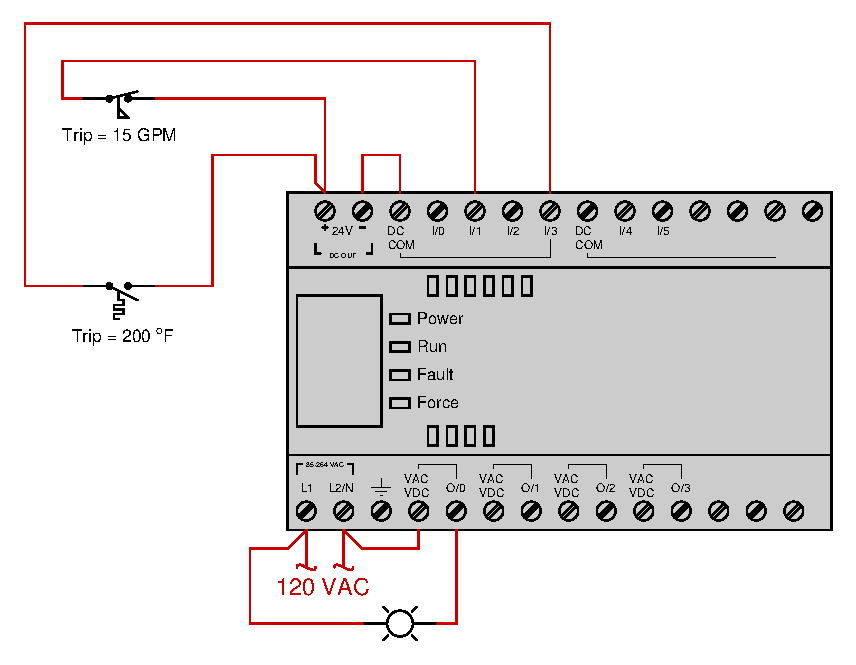
\includegraphics[width=15.5cm]{i02375x01.eps}$$

We wish for the lamp to come on when the temperature is below 200 degrees F {\it and} when the flow rate is below 15 GPM.  Write a RLL program for the PLC (complete with correct address labels for each of the virtual contacts) to fulfill this function:

$$\includegraphics[width=15.5cm]{i02375x02.eps}$$

\vfil

\underbar{file i02375}
\eject
%(END_QUESTION)





%(BEGIN_ANSWER)

This is a graded question -- no answers or hints given!

%(END_ANSWER)





%(BEGIN_NOTES)

$$\includegraphics[width=15.5cm]{i02375x03.eps}$$

In order to turn the light on, we need to send virtual power to coil {\tt O:0/0}.  The ``and'' condition implies a series pairing of contact instructions tied to the two inputs {\tt I:0/1} and {\tt I:0/3}.  Thus, these two contact instruction must both be closed (colored).  Since we are told the temperature will be below 200 degrees (keeping the N.O. temp switch contact in its open state) and that the flow will be below 15 GPM (keeping the N.C. flow switch contact in its closed state), we know that {\tt I:0/3} will be equal to 0 and {\tt I:0/1} will be equal to 1.  In order for the two contact instructions to be colored, we need a NO {\tt I:0/1} and a NC {\tt I:0/3} as shown above.

%INDEX% PLC, ladder logic programming: sketching a solution to a problem

%(END_NOTES)


